\documentclass[letterpaper, 11pt]{article}

\usepackage{amsmath, amssymb, amsfonts}
\usepackage{bm}
\usepackage[dvips]{graphicx}

\newcommand{\pdiff}[2]{\frac{\partial #1}{\partial #2}}

\title{The Stommel Box Model}
\author{Marshall Ward}

\begin{document}

\maketitle

%%%%%%%%%%%%%%%%%%%%%%%%%%%%%%%%%%%%%%%%%%%%%%%%%%%%%%%%%%%%%%%%%%%%%%%%%%%%%%%

\section{Introduction}

This model gives a simple description and dynamics of the Stommel box model. We first provide a physical motivation for the model and derive the dynamical equations. We then consider the equilibrium solutions of this system. Finally, we compare these results to numerical results, and provide a physical interpretation for the solutions.

%%%%%%%%%%%%%%%%%%%%%%%%%%%%%%%%%%%%%%%%%%%%%%%%%%%%%%%%%%%%%%%%%%%%%%%%%%%%%%%

\section{Description of Model}

We consider two well-mixed boxes that have temperatures $T_1$, $T_2$ and salinities $S_1$, $S_2$. The boxes are connected by pipes on the top and bottom, where the flow (that is, a volume flux) in the top is given by $q$; positive $q$ denotes a flow from Box 2 into Box 1. By mass conservation, the flow through the bottom pipe is $-q$.

Since the rate of relaxation for temperature is many orders of magnitude faster than the rate of relaxation for salt, we will presume that the temperatures of the boxes are essentially fixed at some equilibrium values, with a temperature difference of $\Delta T \equiv T_2 - T_1$. Any deviations from these values due to, say, advection of heat between the boxes are presumed to decay so rapidly that they may be neglected. By thinking of Box 2 as equatorial and Box 1 as polar, we may say that $\Delta T > 0$. For salinity, we introduce a fixed forcing term to model an evaporative process, so that the flux on the equatorial box, $E$, is balanced by a reversed flux (or precipitation) in the polar box, $-E$. We further assume that $E > 0$, since we expect evaporation in the tropics and precipitation in the polar regions.

We also allow for the advection of salinity between boxes. Because of the discretized nature of the system, due to the localized mixing of the boxes, the flux into each box depends on the direction of flow. For the upper pipe, if $q > 0$, then Box 2 is losing salinity at a rate $-q S_2 = -|q| S_2$, while Box 1 is gaining this same amount, $|q| S_2$. However, if $q < 0$, then Box 2 is now gaining salinity at a rate $|q| S_1$ while Box 1 loses this its salinity at a rate $-|q| S_1$. If we apply similar logic to the bottom pipe, and also introduce the externally forced fluxes due to evaporation, then the rate of change in $S_1$ and $S_2$ due to salinity are
\begin{align*}
\dot{S}_1 &= -E + |q|(S_2 - S_1) \\
\dot{S}_2 &=  E + |q|(S_1 - S_2)
\end{align*}

For the flow $q$, we presume that there is no relaxation and that it is always driven in response to the buoyant forcing. This is most easily applied to the bottom pipe, where we might expect it to be driven by the differences in hydrostatic pressure between boxes, especially if the boxtops are (open) free surfaces. If $T_2 > T_1$, then the pressure in Box 1 will be heavier and we would expect an induced bottom flow from Box 1 to Box 2, or $q > 0$. Similarly, if $S_2 > S_1$, this would tend to induce a flow from Box 2 to Box 1, or $q < 0$. These results can be phenomenologically combined to give
\begin{equation*}
q = k (\alpha (T_2 - T_1) - \beta (S_2 - S_1))
\end{equation*}
where $k$ is some constant of proportionality. One could argue that this constant is related to a frictional drag parameter $r$, where the frictional pipe drag $\mathcal{F} \equiv r q$ is assumed to be directed from Box 2 to Box 1 when $q > 0$ (since the bottom pipe flow would be from Box 1 to Box 2), and that at all times this remains balanced by the pressure difference $P_1 - P_2 \propto (\alpha(T_2 - T_1) + \beta(S_2 - S_1))$, itself directed from Box 1 to Box 2 when $P_1 > P_2$. In any case, we see that for $\Delta T > 0$, $q > 0$ corresponds to a flow that is principally thermally driven, or \emph{direct cell} flow, while $q < 0$ corresponds to a principally salinity driven flow, or an \emph{indirect cell} flow.

If we therefore combine these results together, then we have a closed set of equations for our system:
\begin{subequations}
\begin{align}
\dot{S}_1 &= -E + |q|(S_2 - S_1) \\
\dot{S}_2 &=  E + |q|(S_1 - S_2) \\
q &= k (\alpha \Delta T - \beta (S_2 - S_1))
\end{align}
\end{subequations}
The equation for $S_2$ is actually somewhat redundant, since we have constructed this model in a way that conserves total salinity, so that $\dot{S_1} + \dot{S_2} = 0$.

%%%%%%%%%%%%%%%%%%%%%%%%%%%%%%%%%%%%%%%%%%%%%%%%%%%%%%%%%%%%%%%%%%%%%%%%%%%%%%%

\section{Model Dynamics}

We now look at a simple analysis of the dynamics of this model. First, we nondimensionalize the equations as such:
\begin{subequations}
\begin{align*}
q &\equiv \left(k \alpha \Delta T\right) q' \\
S_i &\equiv \left(\frac{\alpha \Delta T}{\beta}\right) S_i' \\
E &\equiv \left(\frac{k (\alpha \Delta T)^2}{\beta}\right) E' \\
t &\equiv \left(\frac{1}{k \alpha \Delta T}\right) t'
\end{align*}
\end{subequations}
Then, after dropping the primes, our system becomes
\begin{subequations}
\begin{align}
\dot{S_1} &= -E + |q|(S_2 - S_1) \\
\dot{S_2} &=  E + |q|(S_1 - S_2) \\
q &= 1 - (S_2 - S_2)
\end{align}
\end{subequations}

To further simplify this, we introduce the variable $\delta = S_2 - S_1$. We can then use a single differential equation to describe the dynamics of the box model,
\begin{equation}
\dot{\delta} = 2E - 2 \delta |1 - \delta|
\end{equation}
or equivalently,
\begin{equation}
\dot{q} = -2 E + 2 |q| (1 - q)
\end{equation}

There are at most three equilibrium solutions, namely
\begin{equation}
\delta = \frac{1 \pm \sqrt{1 - 4E}}{2}, \ \frac{1 - \sqrt{1 + 4E}}{2}.
\end{equation}
or equivalently,
\begin{equation}
q = \frac{1}{2} (1 \mp \sqrt{1 - 4E}), \ -\frac{1}{2} (\sqrt{1 + 4E} - 1)
\end{equation}
Note that if $E > 1/4$, then only the last root corresponds to a physical equilibrium. We see that, for $E > 0$, the first two $E$-dependent solutions correspond to direct cells, while the permanent third solution corresponds to an indirect cell.

We now consider the linear stability of each of these points. If $q = \overline{q} + q'$ where $\overline{q}$ is some equilibrium solution, then the linearized dynamics obey
\begin{equation}
\dot{q}' = \left[ 2 \ \mathrm{sgn}(\overline{q}) - 4 |\overline{q}| \right] q'
\end{equation}
where $\mathrm{sgn}$ denotes the sign of the quanity and the results $|\overline{q} + q'| \approx |\overline{q}| + \ \mathrm{sgn}(\overline{q}) q'$ and $\mathrm{sgn}(\overline{q}) \overline{q} = |\overline{q}|$ were used. Each equilibrium solution is then stable as long as $\mathrm{sgn}(\overline{q}) - 2|\overline{q}| < 0$. We therefore find that the indirect cell and the stronger direct cell, 
\begin{equation*}
\overline{q} = -\frac{1}{2} \left( \sqrt{1 + 4E} - 1\right), \ \frac{1}{2} \left(1 + \sqrt{1 - 4E} \right)
\end{equation*}
are stable, while the weaker direct cell
\begin{equation*}
\overline{q} = -\frac{1}{2} \left(1 - \sqrt{1 - 4E}\right)
\end{equation*}
is unstable. Since the differential equation is one dimensional, these linear stability results can be extended to the nonlinear case, and can be taken as general conditions for stability.

%%%%%%%%%%%%%%%%%%%%%%%%%%%%%%%%%%%%%%%%%%%%%%%%%%%%%%%%%%%%%%%%%%%%%%%%%%%%%%%

\section{Results}

We now illustrate some of the theoretical results shown in the previous section. We use a simple Euler method to numerically solve the differential equation in time. We focus on the time evolution of flow strength, $q(t)$.

\begin{figure}[p]
\begin{center}
\resizebox{0.8\textwidth}{!}{
\includegraphics[angle=-90]{boxplot1.ps}}
\caption{Evolution of flow strength for different evaporative forcings}
\end{center}
\end{figure}

Figure 1 shows the evolution of $q$ for different values above and below the critical (rescaled) evaporation rate $E_\mathrm{crit} = \frac{1}{4}$. We see a direct demonstration of the bifurcation that occurs at $E_\mathrm{crit}$, whereby solutions approach a direct cell for small values of $E$, but become an indirect cell for larger values of $E$. Assuming that we start at an initial value $q_0 > \frac{1}{2} (1 - \sqrt{1 -4E})$, always true in our case, the thermal convection is sufficient to transport and mix the fluid quickly enough to prevent the evaporative forcing from creating a significant salinity gradient and an indirect cell. In this case, the solution approaches the strong direct cell. But for $E > E_\mathrm{crit}$, the direct cell is not achievable since in this case the imposed thermal convection is never strong enough to suppress the evaporative forcing, regardless of initial cell strength, and the system always equilibriates to a salinity driven indirect cell. The discrete nature of this bifurcation is even more evident in Figure 2, where smaller variations of $E$ are considered.

\begin{figure}[p]
\begin{center}
\resizebox{0.8\textwidth}{!}{
\includegraphics[angle=-90]{boxplot2.ps}}
\caption{Same as Figure 1, but for smaller variations in $E$}
\end{center}
\end{figure}

\begin{figure}[h]
\begin{center}
\resizebox{0.8\textwidth}{!}{
\includegraphics[angle=-90]{boxplot3.ps}}
\caption{Evolution of flow strength for different initial values $q_0$ and evaporative forcing $E$}
\end{center}
\end{figure}

Figure 3 illustrates the stability of each point for $E = 0.2$, where the equilibrium flows correspond to $q \approx 0.72$ and $q \approx -0.17$. We see that for large values of $q_0$, the thermal convection is too strong for the evaporative forcing to take hold, and the fluid is transported between boxes and its salinity effects are mixed together before saline convection can occur. But when $q_0$ is reduced, evaporative forcing has sufficient time to create a significant salinity difference between boxes, and an indirect cell obtains the chance to take hold and dominate the flow.

%%%%%%%%%%%%%%%%%%%%%%%%%%%%%%%%%%%%%%%%%%%%%%%%%%%%%%%%%%%%%%%%%%%%%%%%%%%%%%%

\section{Conclusions}

We see that there is agreement between the analytical theory and numerical solutions of the Stommel box models. It demonstrates that any thermohaline cell has the potential for multiple equilibrium flows, even those that flow in opposite directions. Although the thermohaline circulation of the oceans is undoubtedly more complicated, this model demonstrates that it may possess a similar property. Also, because our current climate is dependent on a direct thermohaline cell, changes in the external forcing may produce a situation similar to that where $E > E_\mathrm{crit}$, so that the only possible flow is an indirect cell, which could have severe implications for our climate. Features such as the effects of nonlinearity and the internal dynamics of each ``box'', as well as the nature of the interaction between the various oceans of the world, may introduce additional features that are more important than this effect illustrated in the Stommel Box Model; they may even completely suppress the process. But it is also possible that such complexity may only cause a slight distortion of this result, and that the effect is preserved and acts as a fundamental component of global climate.

\end{document}